% !TeX root = ../main.tex

\section{Sviluppo Applicazione}

\begin{frame}{Applicazioni Multipiattaforma}

    \textbf{Principio}:
    \begin{itemize}
        \item Condivisione logica applicativa
        \item UI/UX nativa
        \item Assenza di software aggiuntivo di emulazione
    \end{itemize}

    \vspace{3mm}

    \textbf{Vantaggi}:
    \begin{itemize}
        \item Una sola base di codice per la logica applicativa
        \item Meno risorse richieste
        \item Meno codice da manutenere
        \item Utilizzo come dipendenza di progetto
        \item Rilasci più rapidi
    \end{itemize}
    
\end{frame}

\begin{frame}{Kotlin Multiplatform}
    \begin{columns}[onlytextwidth]
        \begin{column}{0.55\textwidth}
        
             \begin{figure}[H]
                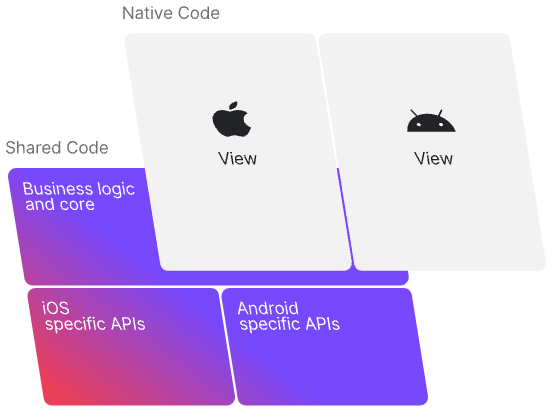
\includegraphics[width=1\textwidth]{img/kmm-stack-official.png}
            \end{figure}
            
        \end{column}
        \begin{column}{0.45\textwidth}
        
            \textbf{Caratteristiche}:
            \begin{itemize}
                \item Framework per lo sviluppo di applicazioni multipiattaforma 
                \item L'utilizzo in ambito mobile è il più diffuso per Android e iOS (Kotlin Multiplatform Mobile)
                \item Ancora non molto maturo (fase ``pre-stable'')
                \item Utilizzato in produzione da aziende come Netflix, Philips e VMware
            \end{itemize}
            
        \end{column}
    \end{columns}
\end{frame}

\begin{frame}{Struttura Applicazione}
    \begin{columns}[onlytextwidth]
        \begin{column}{0.45\textwidth}

            \textbf{Logica Applicativa}:
            \begin{itemize}
                \item Modellazione del dominio (editoria digitale)
                \item Ricerca e download pubblicazioni digitali
                \item Persistenza dei segnalibri, delle annotazioni e dei preferiti
                \item Autenticazione degli utenti abbonati
            \end{itemize}

            \vspace{3mm}

            \textbf{UI Android/iOS}:
            \begin{itemize}
                \item Visualizzazione dati
                \item Lettura pubblicazioni digitali
                \item Gestione input utente
            \end{itemize}
            
        \end{column}
        \begin{column}{0.55\textwidth}
        
             \begin{figure}[H]
                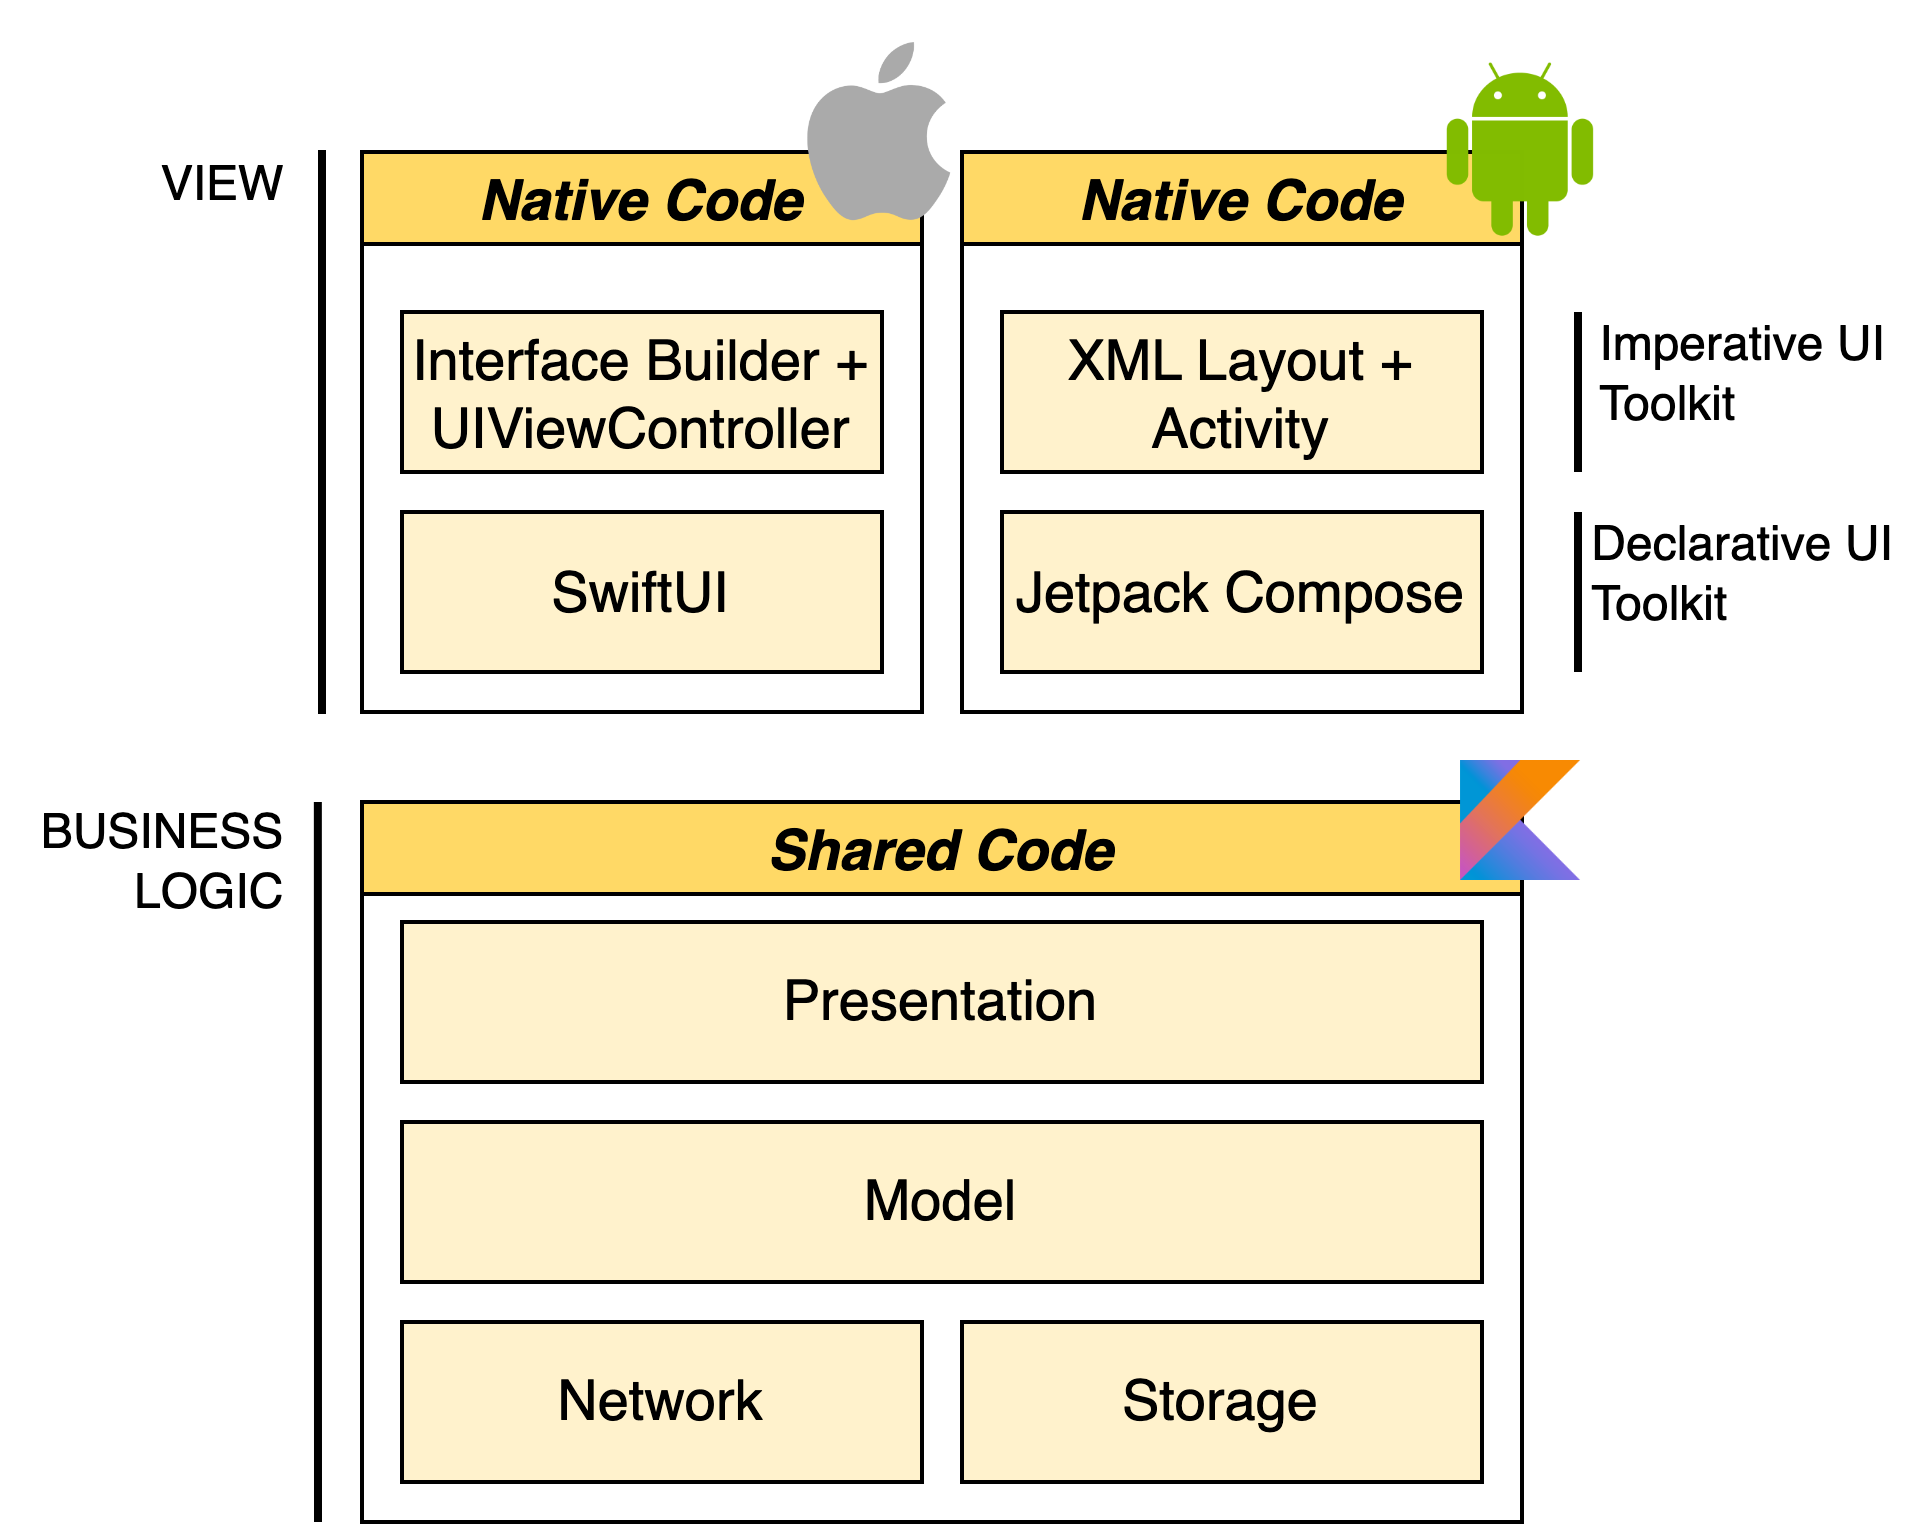
\includegraphics[width=1\textwidth]{img/stack_kmm.png}
            \end{figure}
            
        \end{column}
    \end{columns}
\end{frame}

\begin{frame}{Struttura Applicazione}
    \begin{columns}[onlytextwidth,t]
        \begin{column}{0.4\textwidth}

            \textbf{Kotlin/JVM}
            \begin{itemize}
                \item Input: Codice Kotlin
                \item Output: Libreria Android
            \end{itemize}

            \vspace{4mm}

            \textbf{Kotlin/Native}
            \begin{itemize}
                \item Input: Codice Kotlin
                \item Output: Libreria iOS
            \end{itemize}            
            
        \end{column}
        \begin{column}{0.6\textwidth}
        
             \begin{figure}[H]
                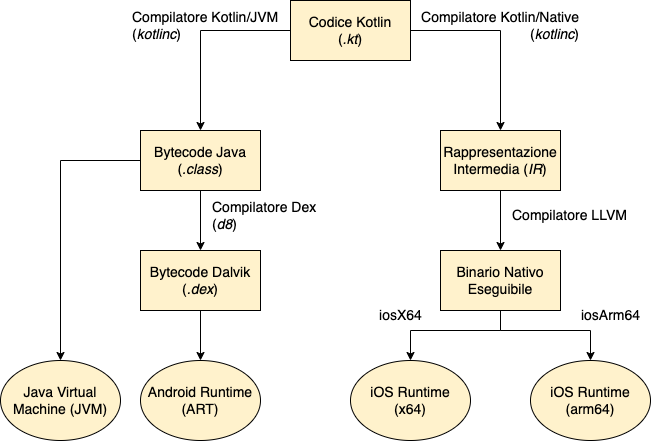
\includegraphics[width=1\textwidth]{img/compilatore_kotlin.png}
            \end{figure}
            
        \end{column}
    \end{columns}
\end{frame}

\begin{frame}{UI Android}
    \begin{columns}[onlytextwidth]
        \begin{column}{0.24\textwidth}
        
            \begin{figure}[H]
                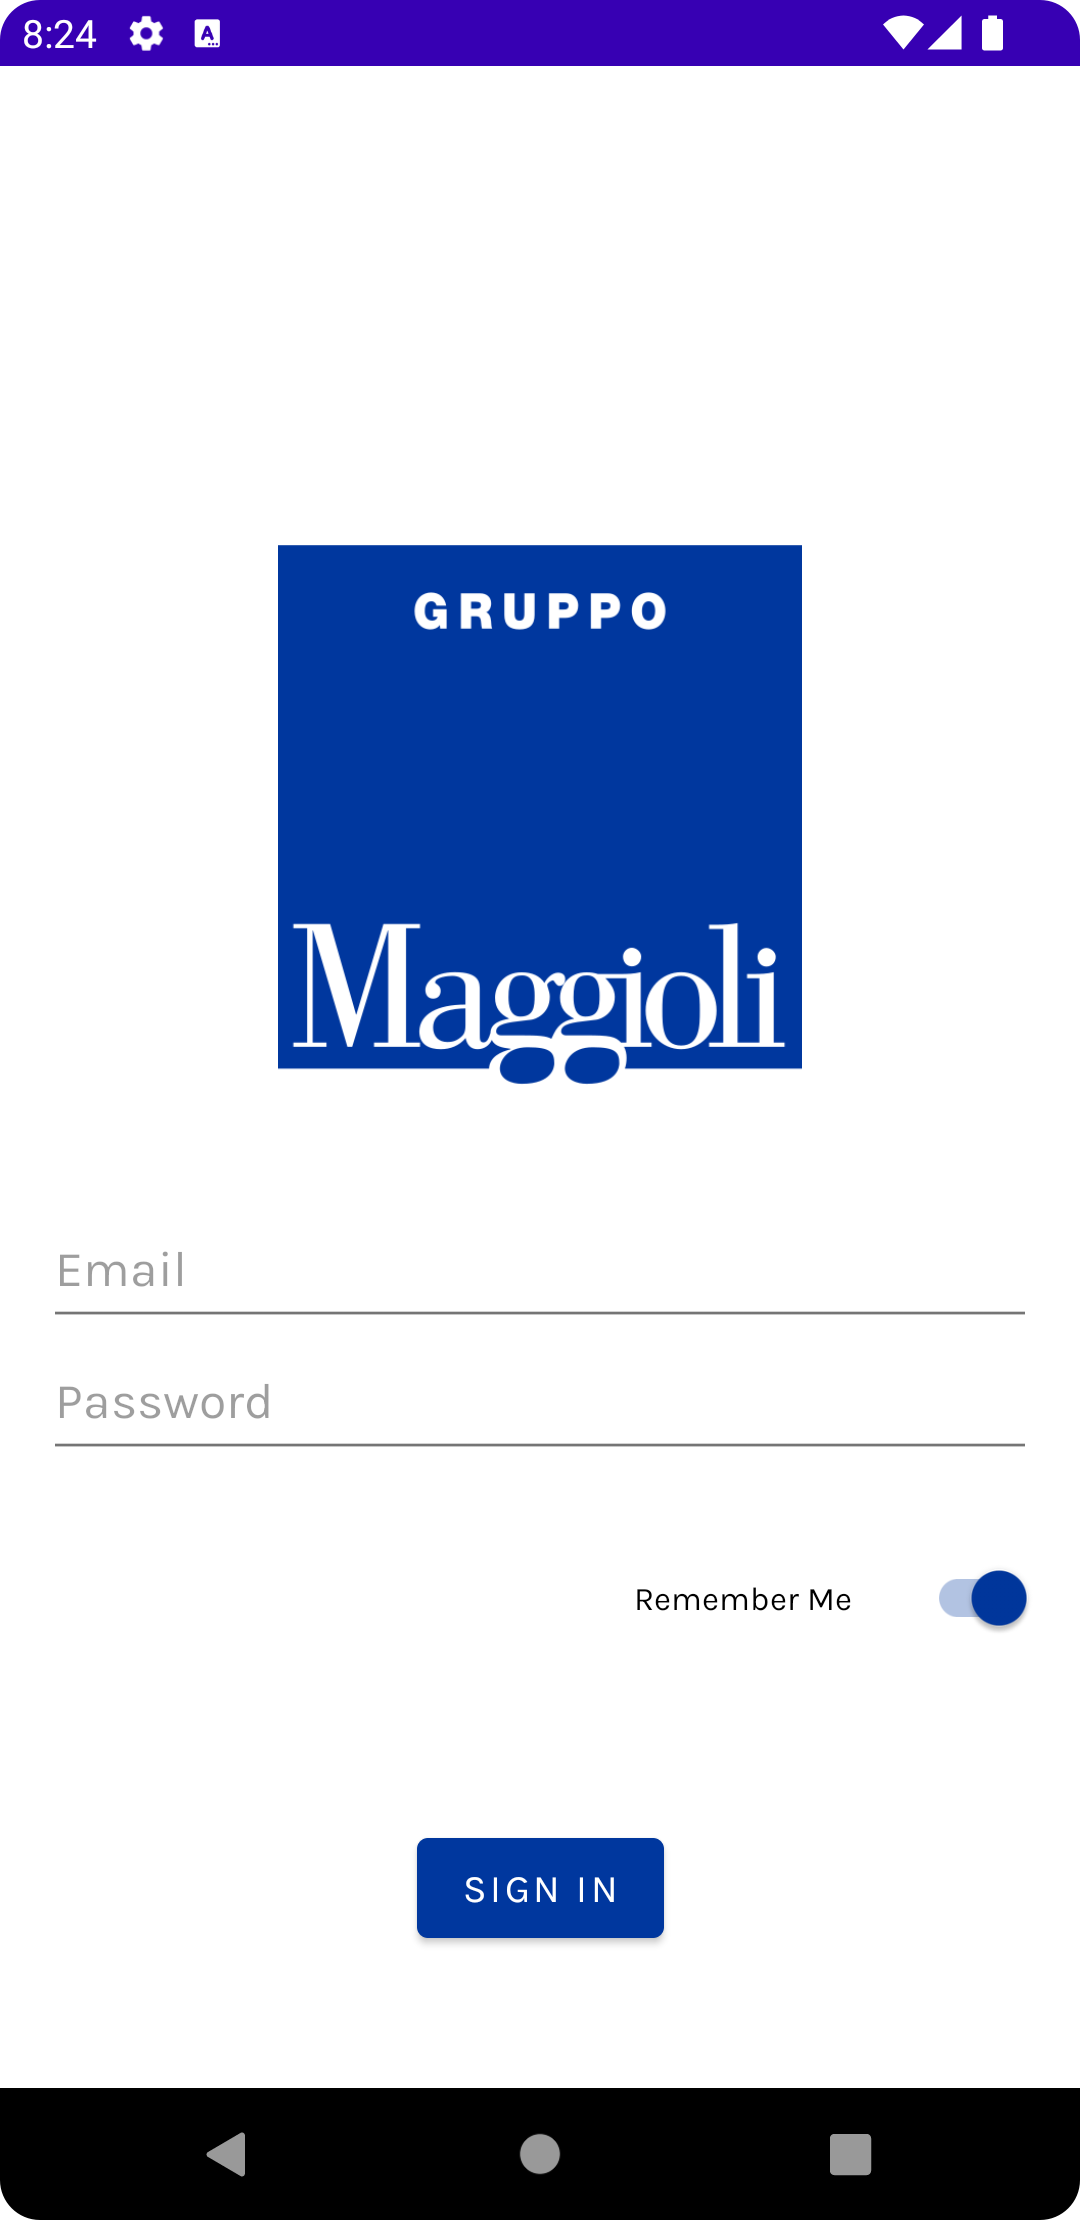
\includegraphics[width=1\textwidth]{img/login.png}
            \end{figure}
            
        \end{column}
        \begin{column}{0.24\textwidth}
        
            \begin{figure}[H]
                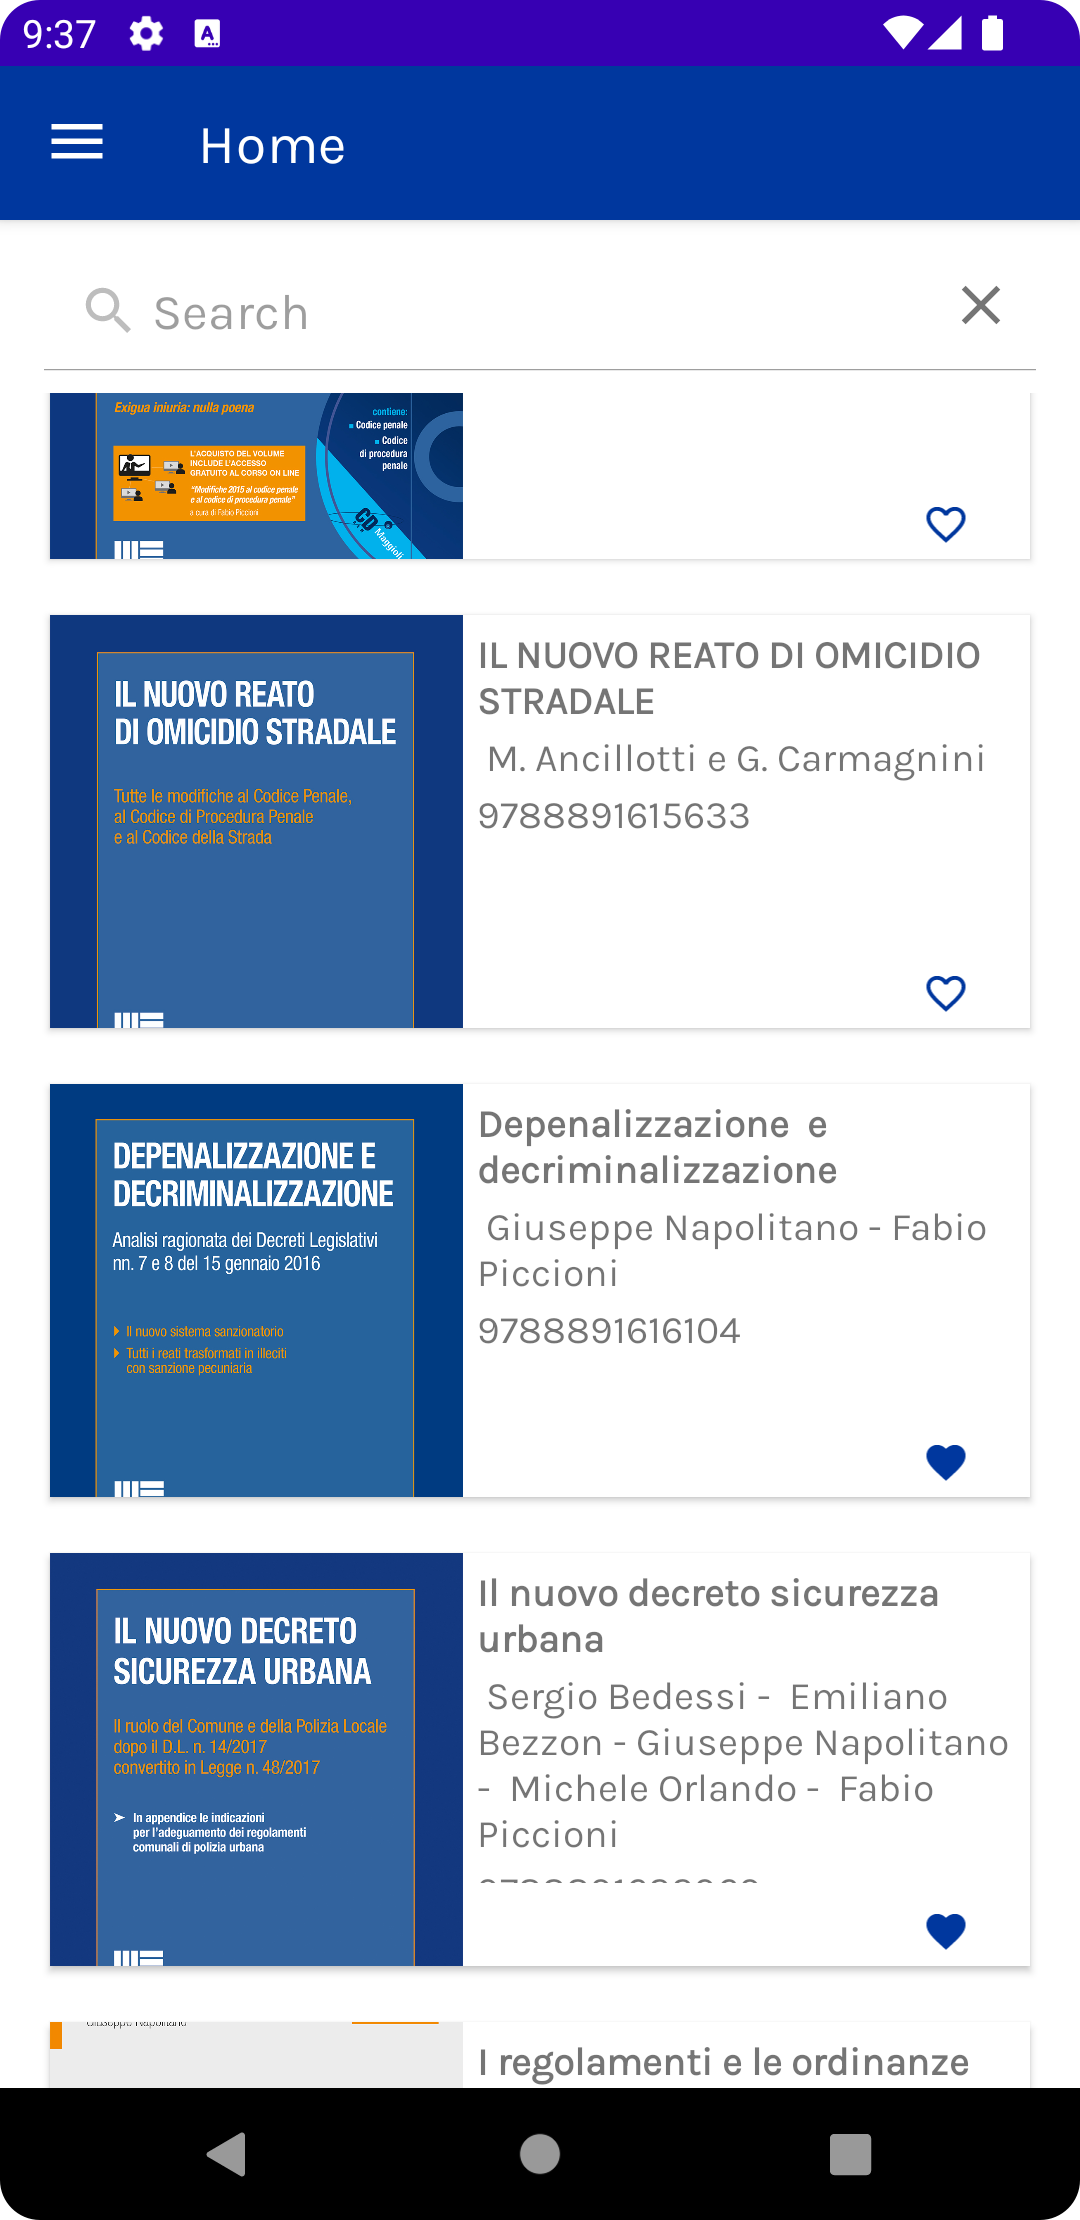
\includegraphics[width=1\textwidth]{img/home.png}
            \end{figure}
            
        \end{column}
        \begin{column}{0.24\textwidth}
        
            \begin{figure}[H]
                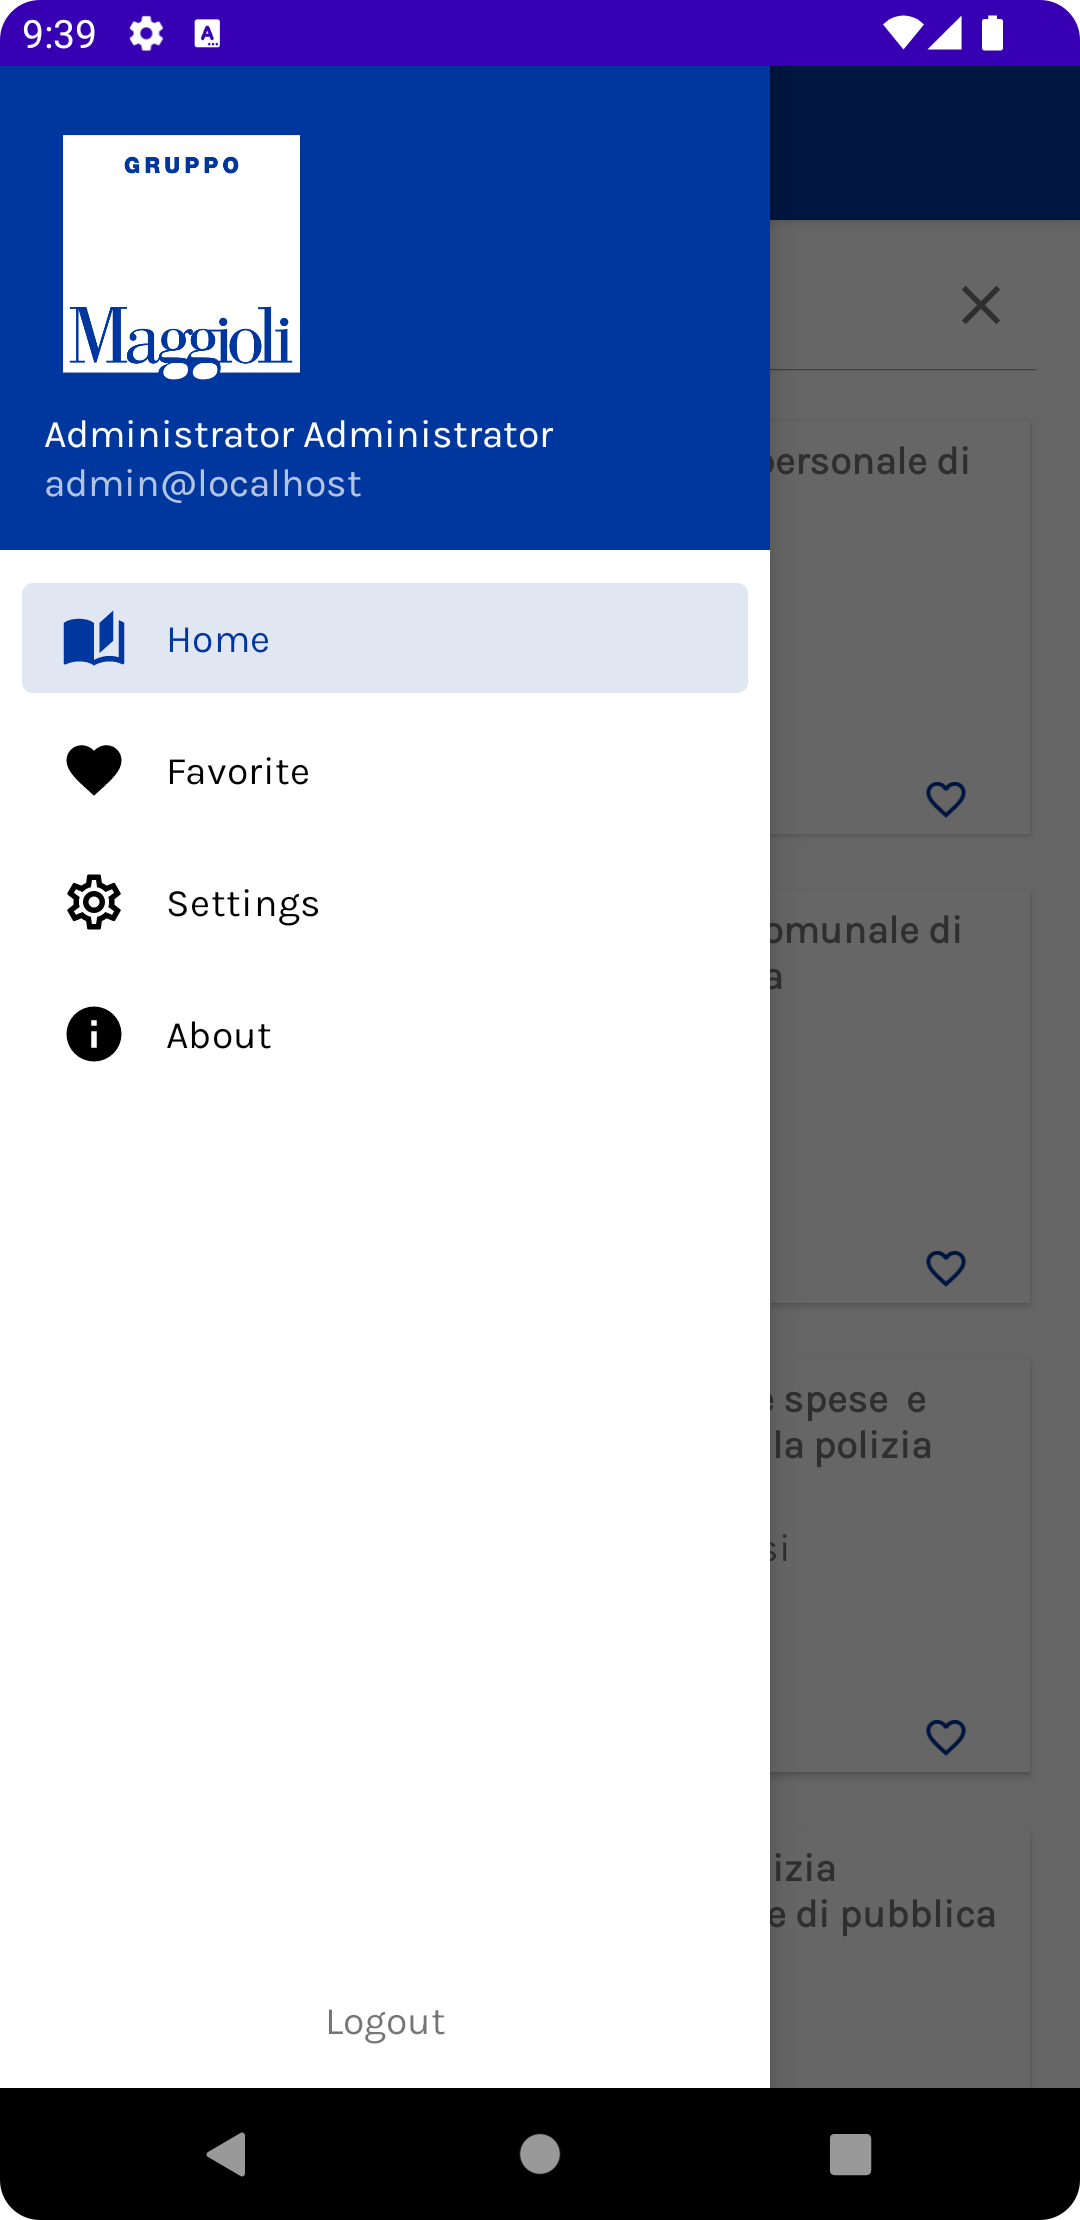
\includegraphics[width=1\textwidth]{img/sidenav.png}
            \end{figure}
            
        \end{column}
        \begin{column}{0.24\textwidth}
        
            \begin{figure}[H]
                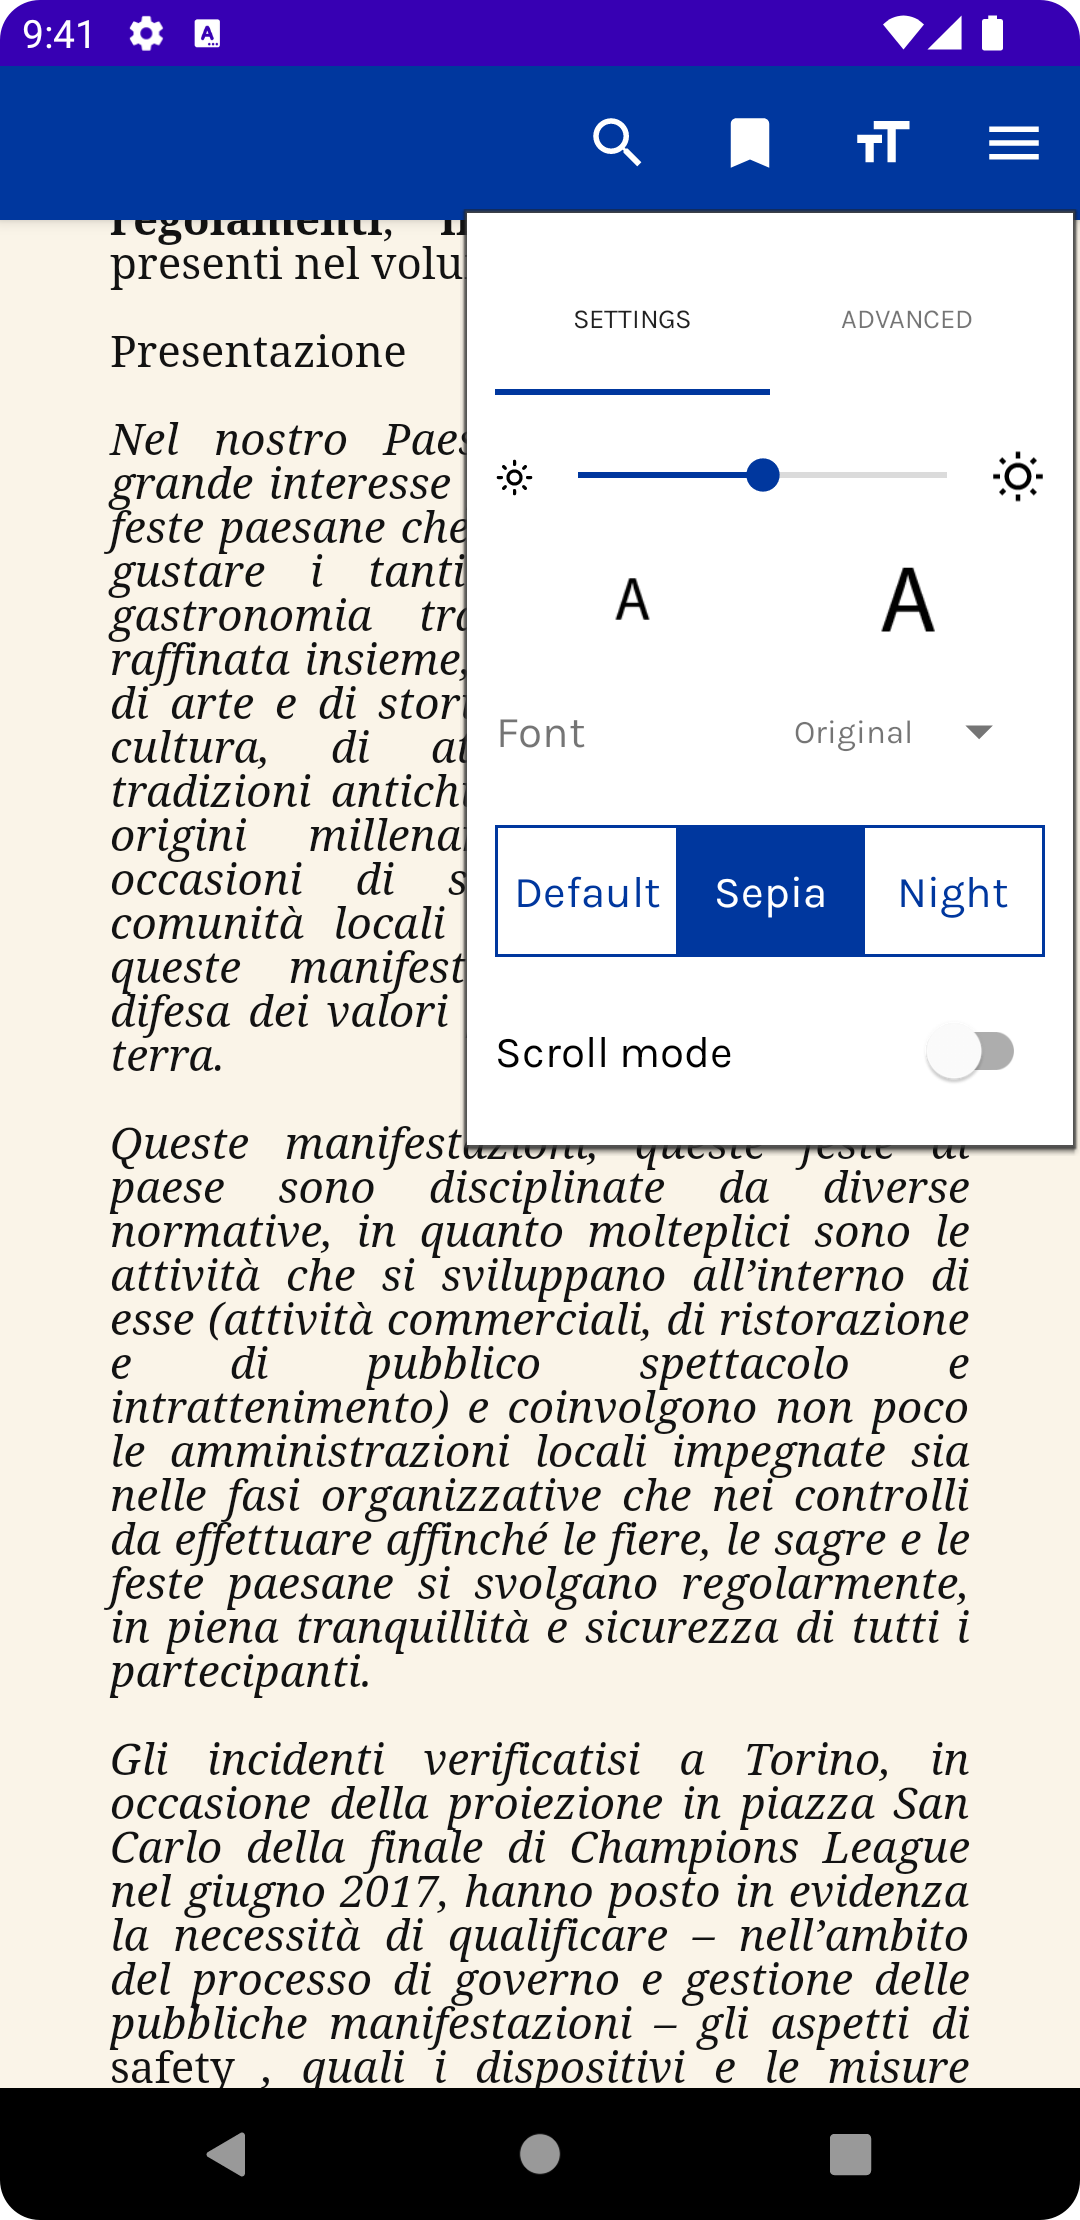
\includegraphics[width=1\textwidth]{img/reader_settings.png}
            \end{figure}
            
        \end{column}
    \end{columns}
\end{frame}

\begin{frame}{UI iOS}
    \begin{columns}[onlytextwidth]
        \begin{column}{0.24\textwidth}
        
            \begin{figure}[H]
                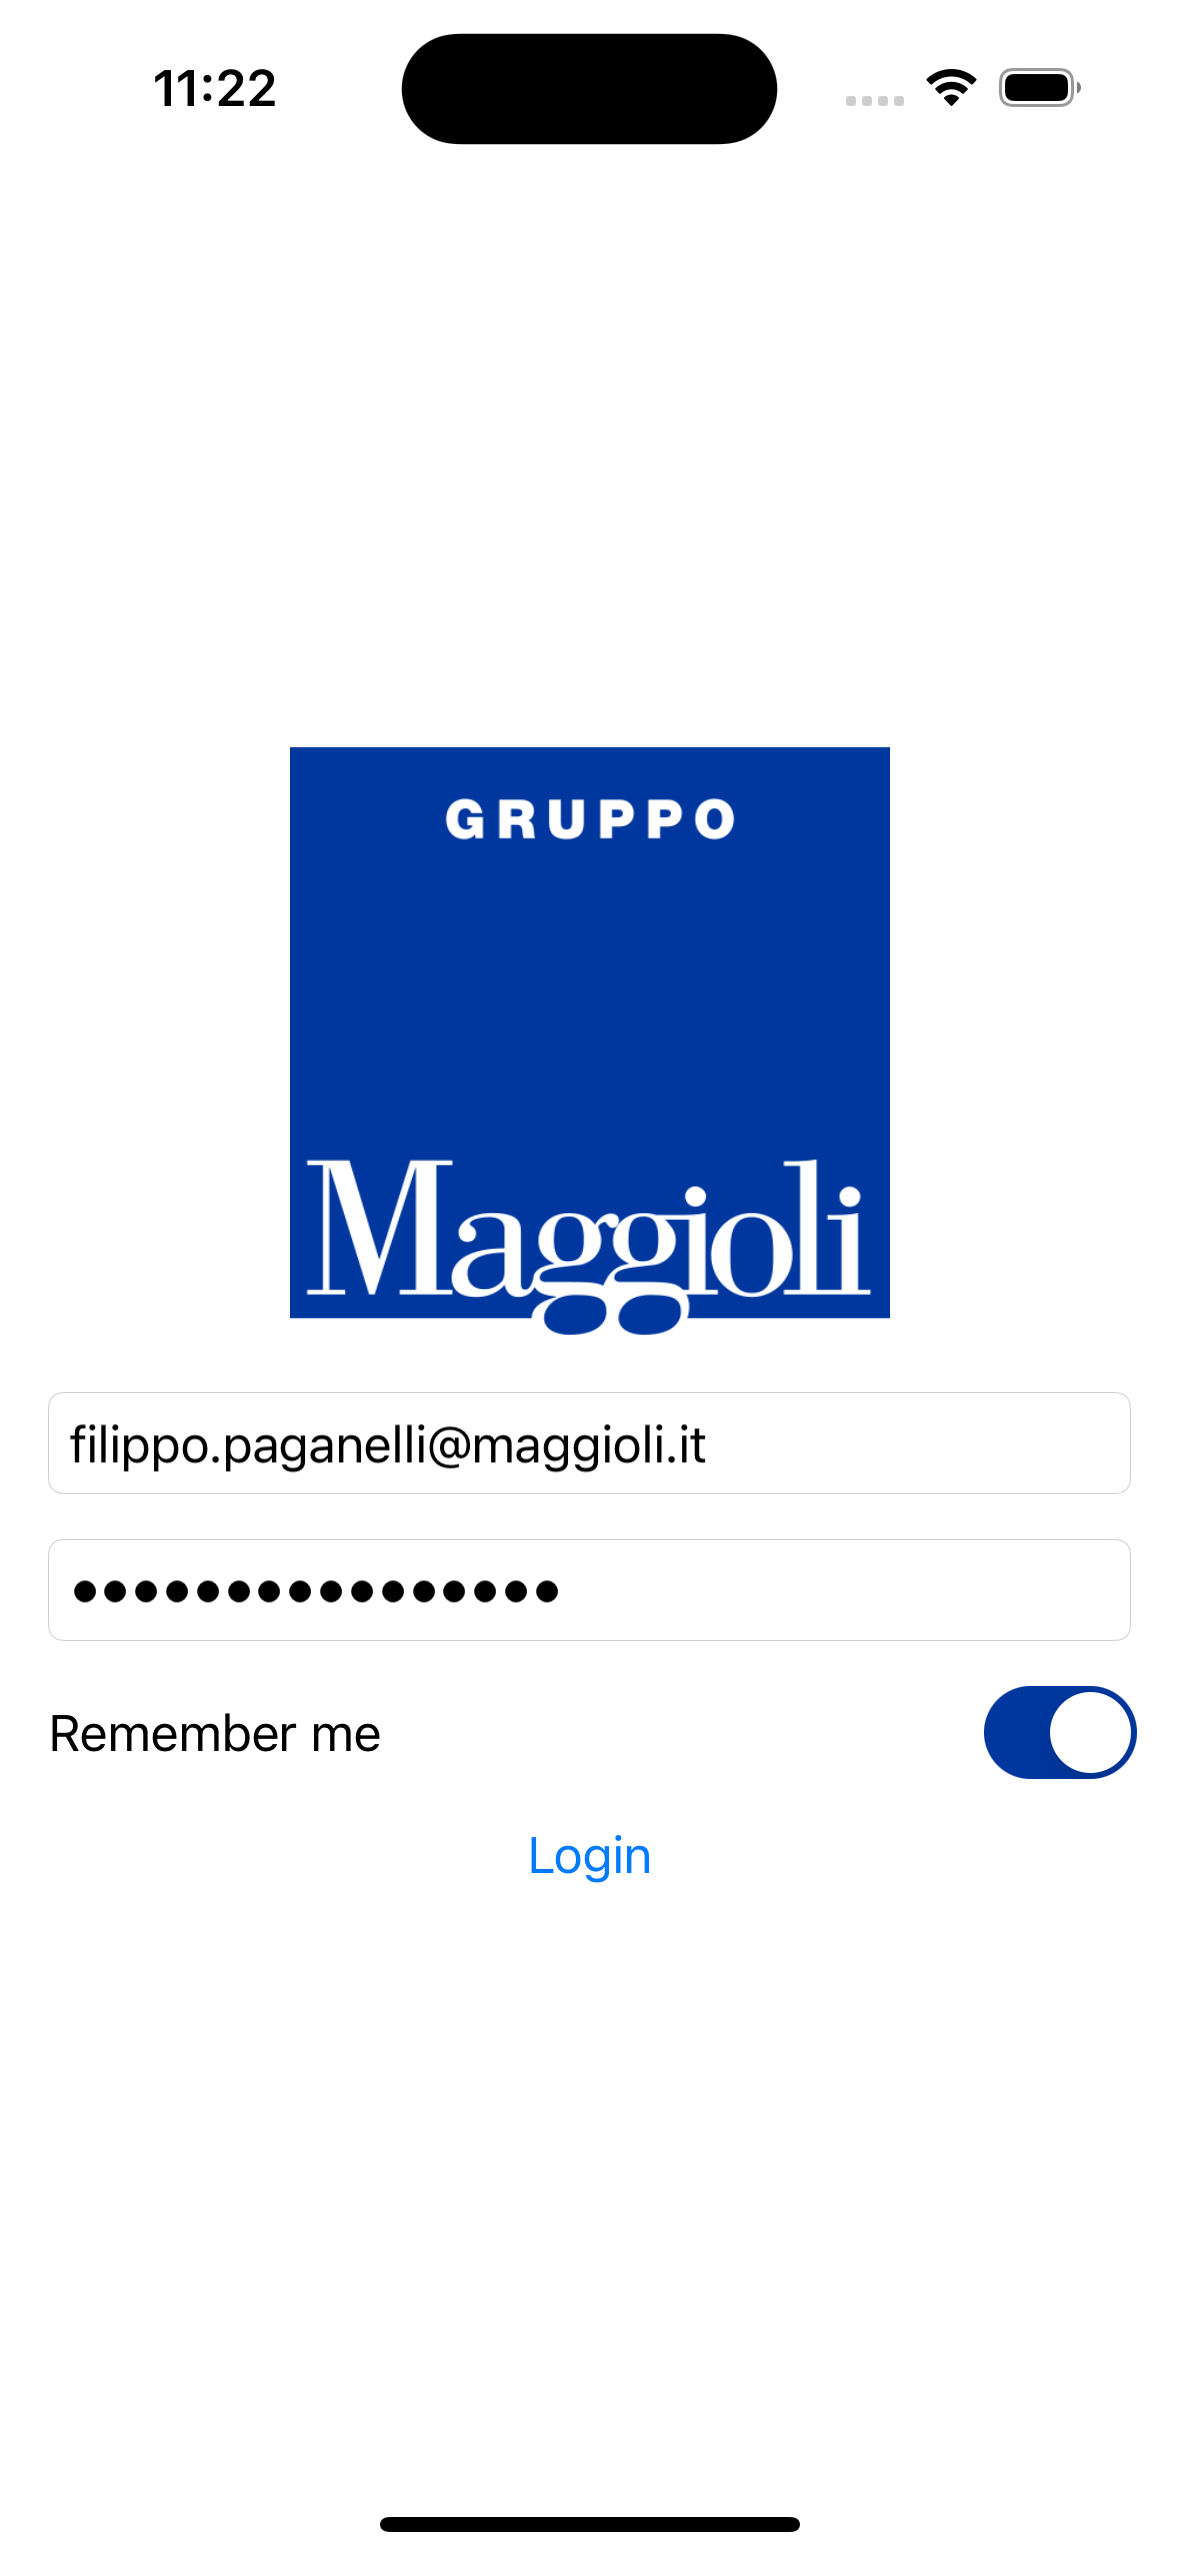
\includegraphics[width=1\textwidth]{img/login_ios.png}
            \end{figure}
            
        \end{column}
        \begin{column}{0.24\textwidth}
        
            \begin{figure}[H]
                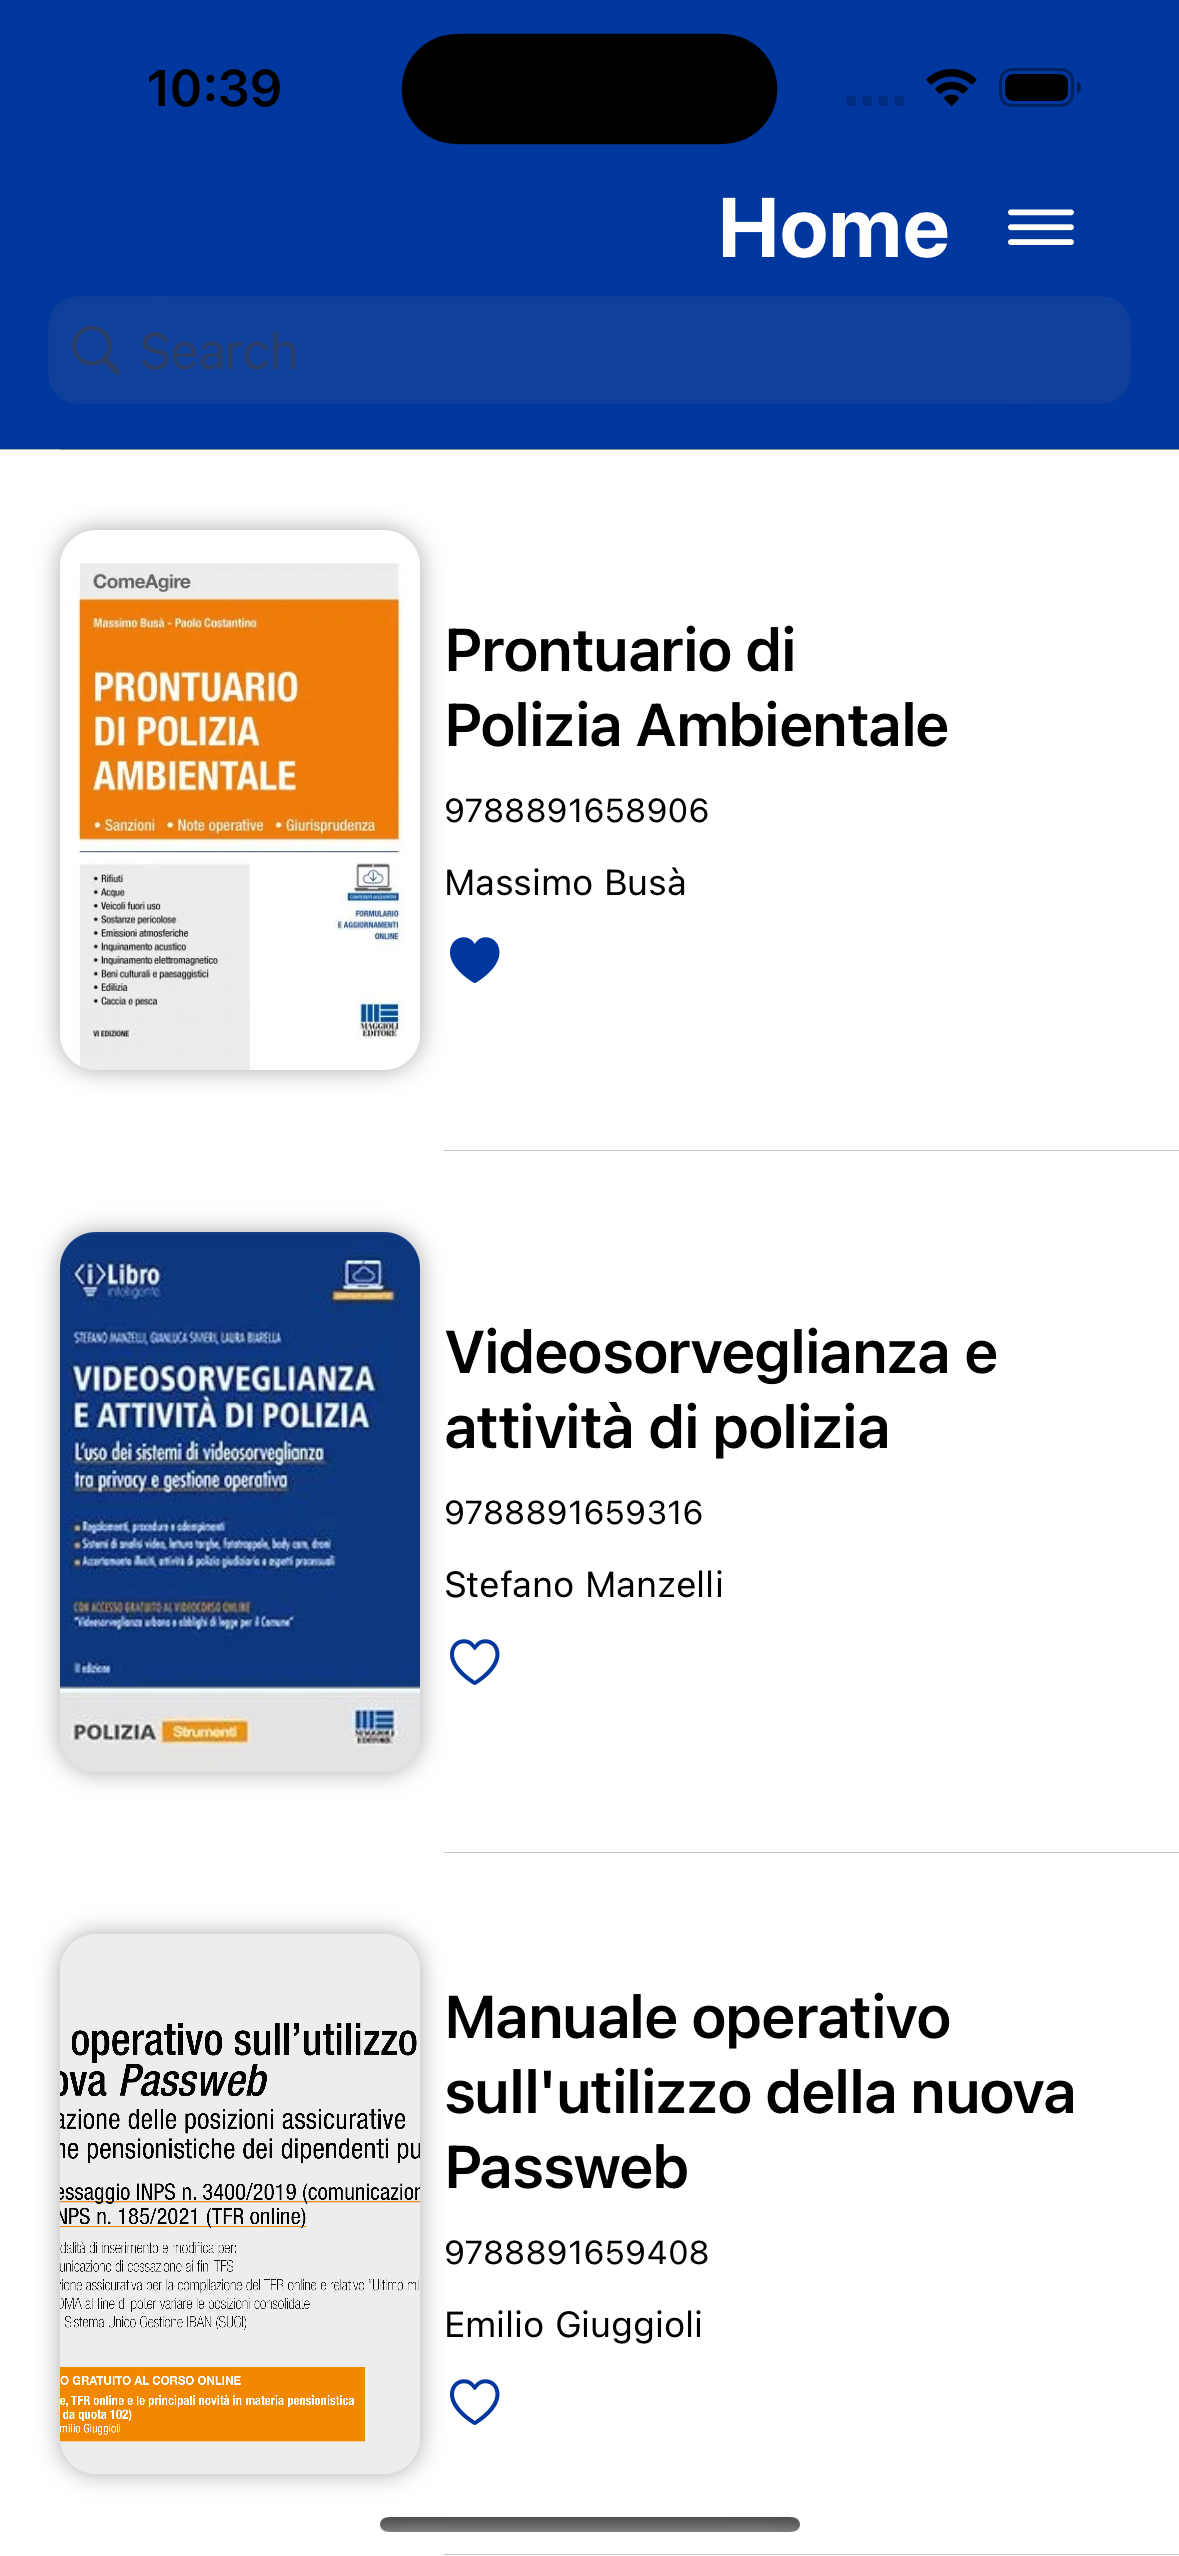
\includegraphics[width=1\textwidth]{img/home_ios.png}
            \end{figure}
            
        \end{column}
        \begin{column}{0.24\textwidth}
        
            \begin{figure}[H]
                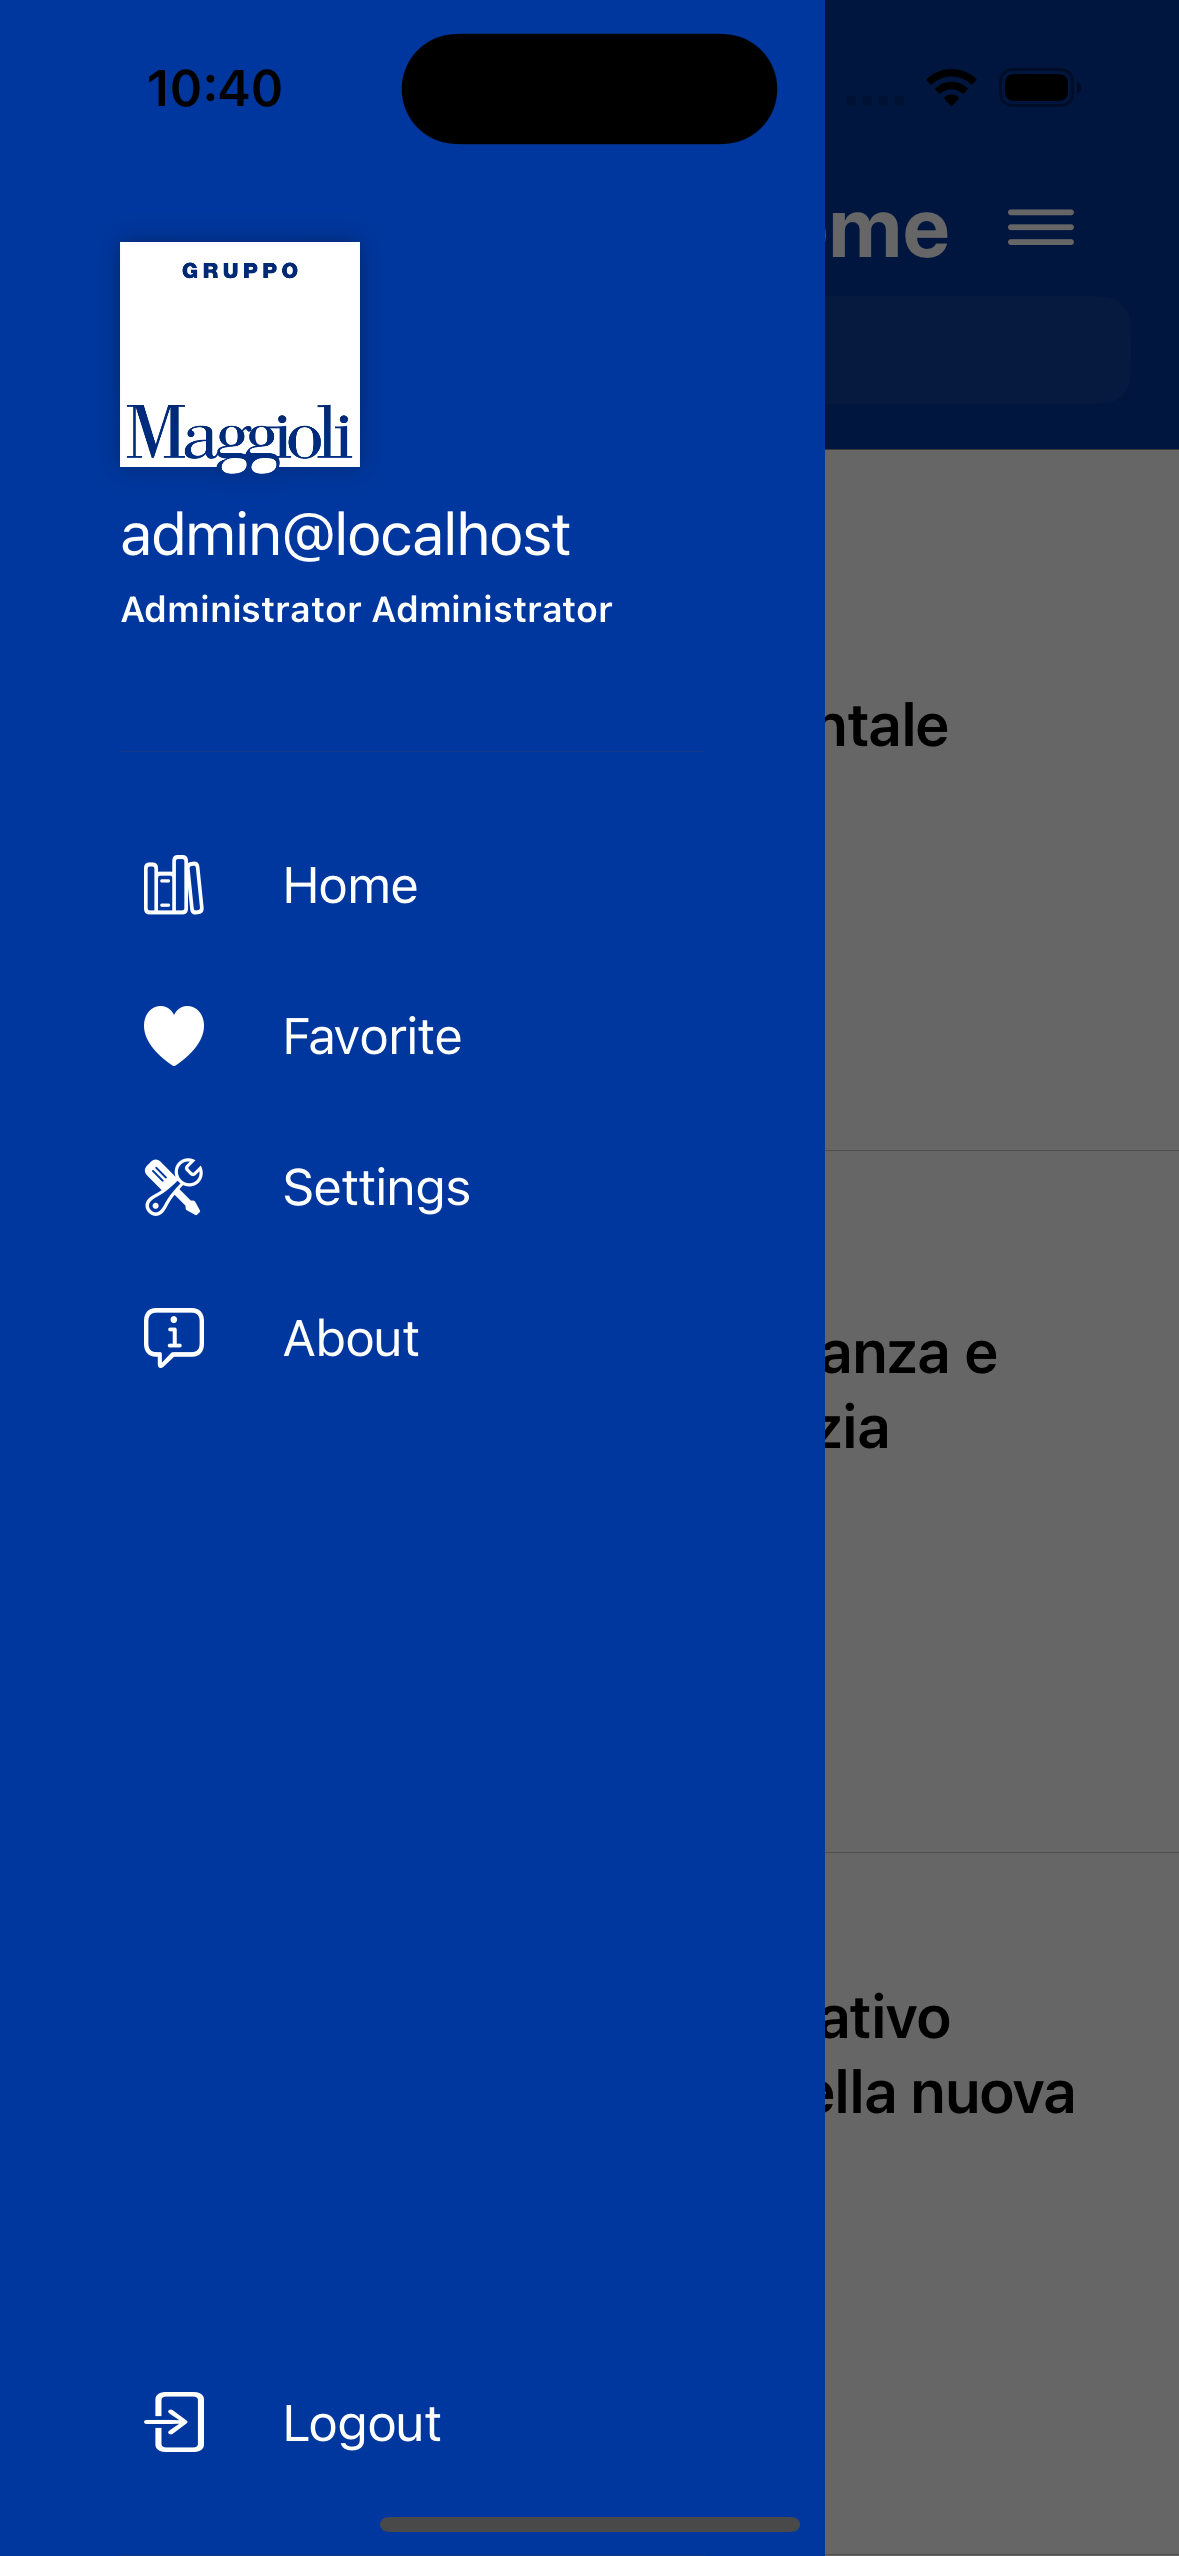
\includegraphics[width=1\textwidth]{img/sidenav_ios.png}
            \end{figure}
            
        \end{column}
        \begin{column}{0.24\textwidth}
        
            \begin{figure}[H]
                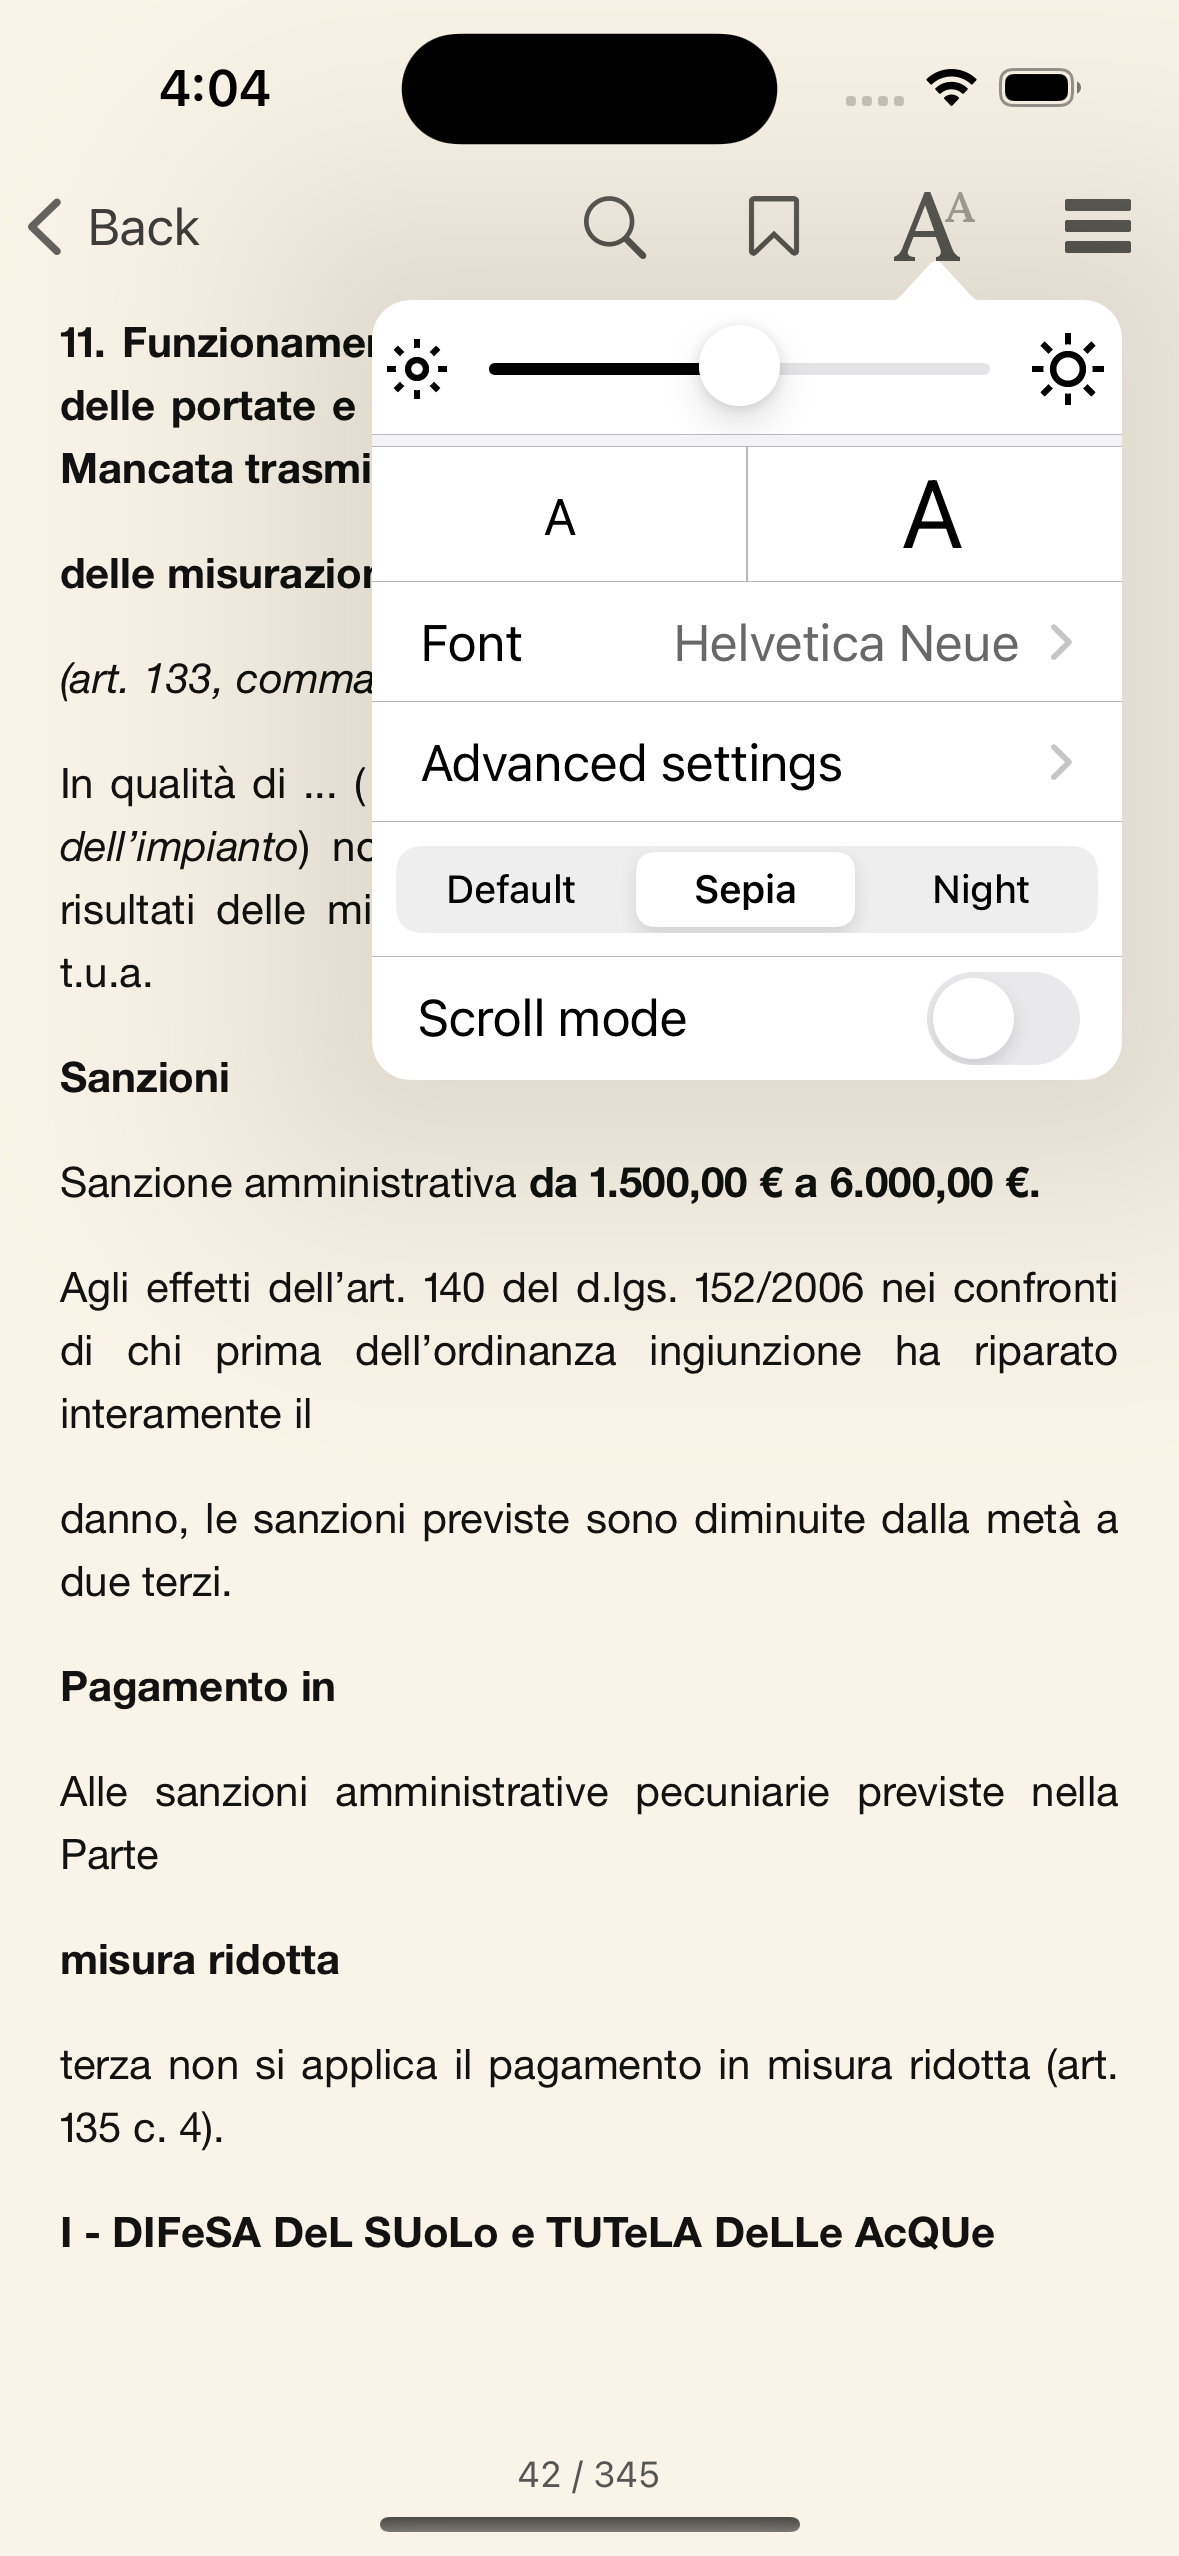
\includegraphics[width=1\textwidth]{img/reader_settings_ios.png}
            \end{figure}
            
        \end{column}
    \end{columns}
\end{frame}
